\documentclass{article}
\usepackage{subcaption}% for subfigures
\usepackage[%  
    colorlinks=true,
    pdfborder={0 0 0},
    linkcolor=blue
]{hyperref}% for hyperlinkning to figures
\usepackage{graphicx} % Required for inserting images

\title{Simple Linear Regression on Student Marks vs Study Time}
\author{Johnathan Ferdinand, Devina Gera, Archimedes Li, \\ Henry Liu, Katherine Shi, Samuel Stevens}
\date{February 26, 2025}

\begin{document}

\maketitle

\section{Introduction}
Our model is a simple linear regression, which is a function of 1 feature, $X_1$, that predicts a label $\hat{y}$ in the form of $\hat{y} = \beta_1X_1 + \beta_0$.  
The benefits of using a linear regression are its simplicity and high level of explainability.  
This makes it a good candidate for modeling a simple relationship between two variables.  
Therefore, we decided to model the relationship between student marks and time studied taken from the dataset "Student Marks Dataset" which we will discuss further in the Data Description section.
However, a drawback to simple linear regressions are their low complexity.  We selected a dataset that fits these constraints. \\

\noindent The R packages that we used were tidyverse and ggpubr for visualization, lmtest for linear regression diagnostics, caret for linear regression training, and caTools for data analysis and manipulation.

\section{Data Description}
The dataset we used was one called “Student Marks Dataset” from Kaggle, which was sourced from the UCI Machine Learning Repository. The dataset consists of data on 100 different students' marks, study times, and number of courses.  
The features in the dataset are the student’s study time in hours and the number of courses taken by the student.  
The student’s study time ranges from $[0.1, 7.96]$, and the number of courses taken ranges from $[3, 8]$. 
However, because our objective is to implement a simple linear regression model, we decided to only use one feature: study time.
The label is the overall marks of the students, which ranges from $[5.61, 55.3]$.  
A scatter plot for our chosen data is shown below in Figure \ref{fig:scatterplot}. 
The box plots of marks and time studied are shown in Figure \ref{fig:boxplots}. \\

\noindent There are three important observations we make. The first is that as shown in Figure \ref{fig:boxplots}, there are no outliers. Therefore, we decided not to clean the data.
Second, we notice a strong correlation between Marks and time studied in Figure \ref{fig:scatterplot}. \\
And finally, we notice that the distribution of marks (Figure \ref{fig:boxplotMarks}) is skewed left while the distribution of time studied (Figure \ref{fig:boxplotTime}) is symmetric.
\clearpage

\begin{figure}[h]
\centering
    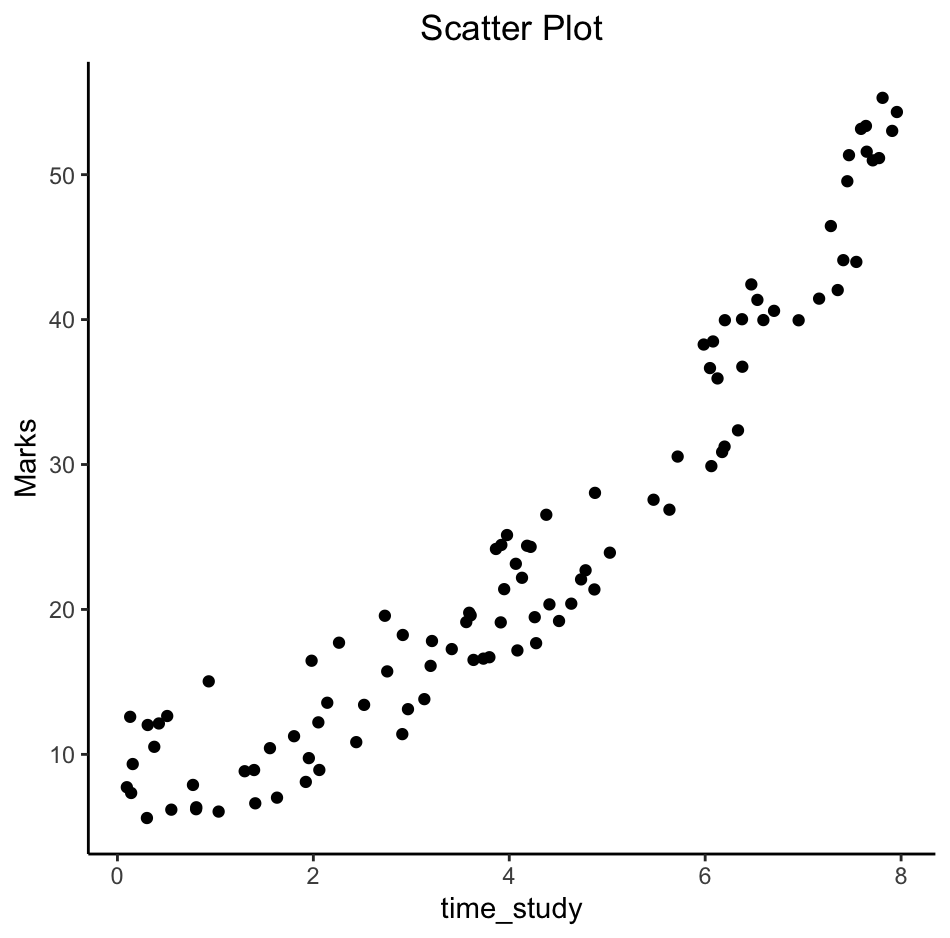
\includegraphics[width=0.4\linewidth]{imgs/Scatter_Plot.png}
    \caption{A scatter plot of marks (y-axis) as a function of hours spent studying (x-axis) }
    \label{fig:scatterplot}
\end{figure}


\begin{figure}[h]
\centering
\begin{subfigure}{0.4\textwidth}
    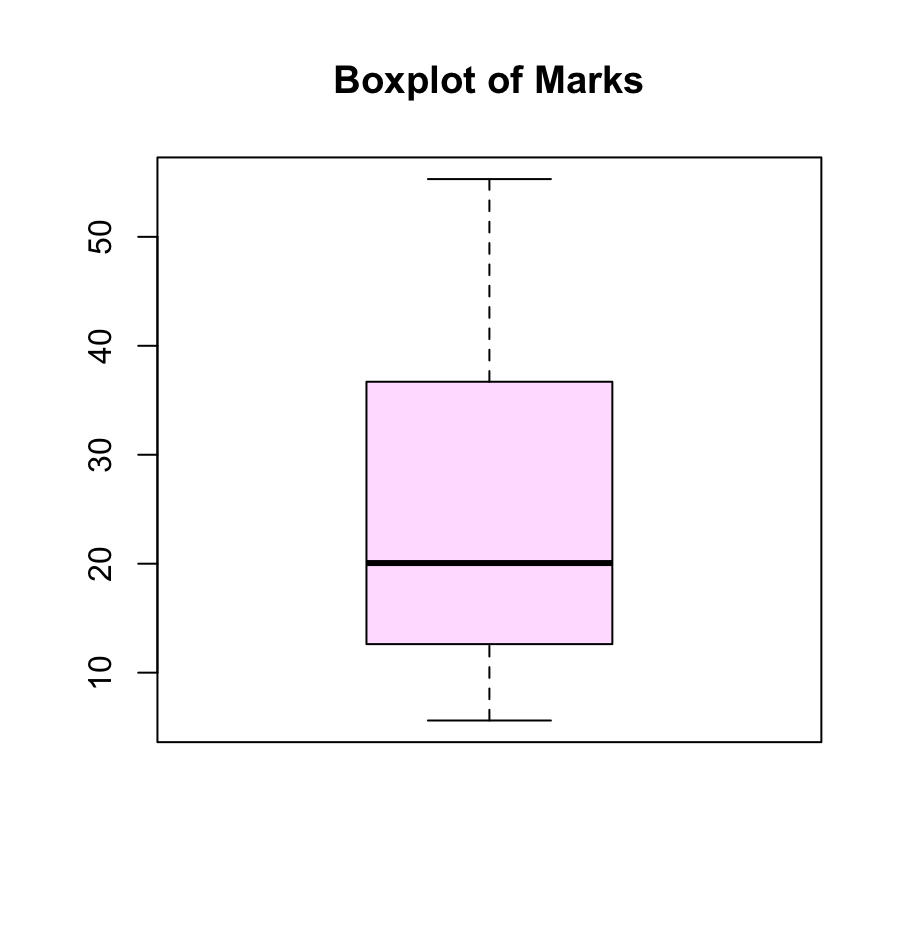
\includegraphics[width=\textwidth]{imgs/Marks_Boxplot.png}
    \caption{}
    \label{fig:boxplotMarks}
    \end{subfigure}
    \hfill
    \begin{subfigure}{0.4\textwidth}
    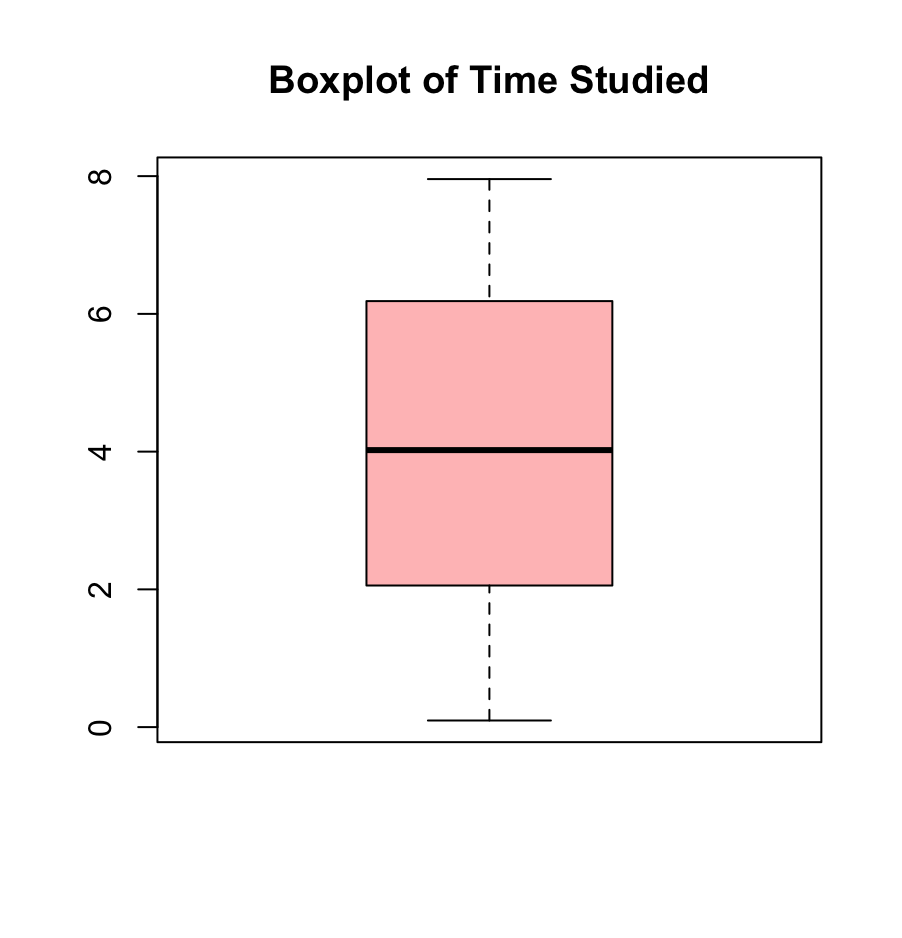
\includegraphics[width=\textwidth]{imgs/Time_Study_Boxplot.png}  
    \caption{}
    \label{fig:boxplotTime}
    \end{subfigure}
    \caption{Box plot of marks (\subref{fig:boxplotMarks}) and time studied (\subref{fig:boxplotTime})}
    \label{fig:boxplots}
\end{figure}

\clearpage

\section{Analysis}

Our dataset of 100 observations was divided into 80\% training data and 20\% testing data using the sample.split function from the caTools package, resulting in 80 observations for training and 20 for testing.\\

\noindent Using the training data, we fitted a simple linear regression model with study time as our single predictor variable. Our fitted model is:
\begin{equation} \hat{y} = 1.2548 + 5.6713X_1 \end{equation}

\noindent Where $X_1$ represents hours studied and $\hat{y}$ represents predicted marks. The coefficient 5.6713 indicates that for each additional hour of study time, a student's marks are expected to increase by approximately 5.67 points.

%someone deal with the cook distance pls
\begin{figure}[h]
\centering
    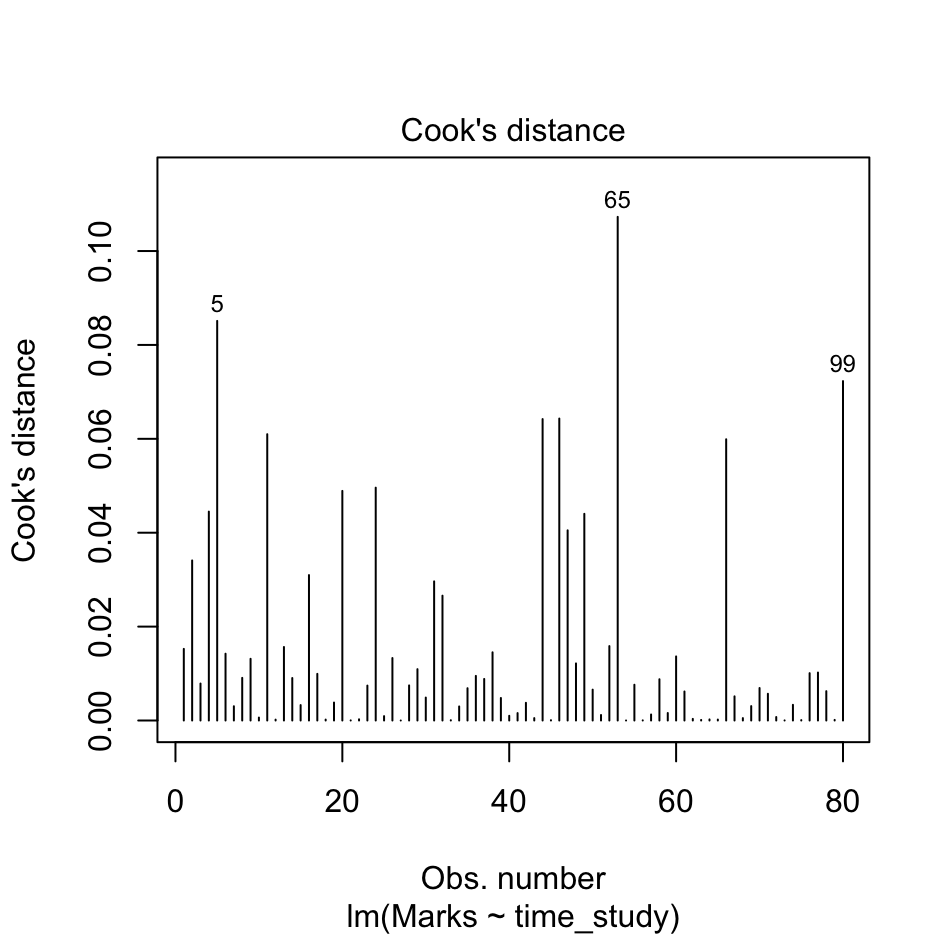
\includegraphics[scale=0.3]{imgs/Cook_Distance.png}    
    \caption{Plot of Cook's distance as a function of observation number}
    \label{fig:cook}
\end{figure}

\noindent This analysis identified observations 5, 65, and 99 as influential points, though we retained them in our model as they appeared to be valid data points rather than errors.\\

% \noindent Our model achieved an $R^2$ value of 0.8882, indicating that approximately 89\% of the variance in student marks can be explained by study time alone. The Root Mean Square Error (RMSE) was 5.42 for the training data and 3.073, showing good generalization. \\

\noindent As shown in the scatter plot (Figure \ref{fig:scatterplot}), there is a strong positive correlation between study time and marks. The boxplots (Figure \ref{fig:boxplots}) reveal that the marks distribution is positively skewed with a median around 20, while the study time distribution is more symmetrical with a median of about 4 hours. \\

\noindent These results confirm our initial visual assessment that study time is a strong predictor of student marks, validating our choice of simple linear regression for modeling this relationship.

\section{Model Evaluation and Prediction}
We find the following values for standardized error and $t$-value for the two coefficients as follows:

\begin{center}
  \begin{tabular}{c | c c}
    & Std Error & t-value \\
    \hline
    $\hat{\beta_0}$ & 1.0802 & 1.162 \\
    $\hat{\beta_1}$ & 0.2278 & 24.893
  \end{tabular}
\end{center}

\noindent On the training data, we found a residual standard error value of $5.025$ on $78$ degrees of freedom. We found a multiple $R^2$ value of $0.8882$ and an $F$-statistic of $619.7$ on $1$ predictor and $78$ degrees of freedom. \\

\noindent Our regression model compared with the test set data points appears as follows (Figure \ref{fig:testsSet}):

\begin{figure}[h]
    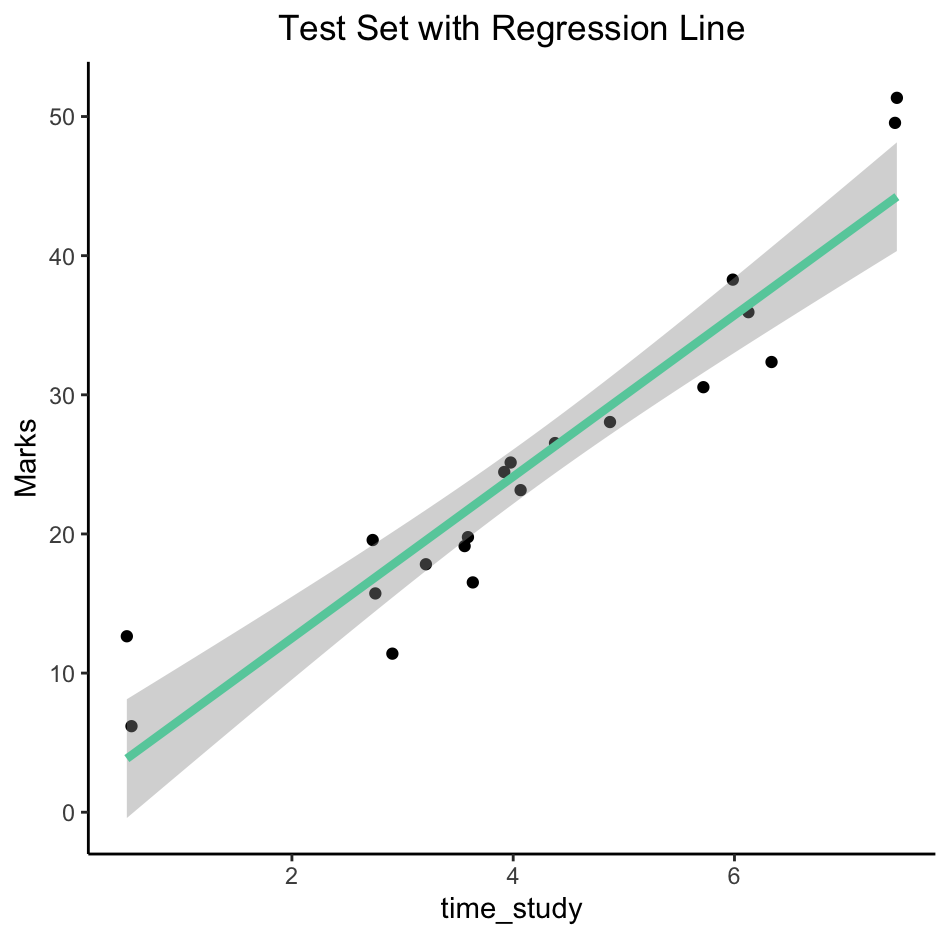
\includegraphics[width=0.75\linewidth]{imgs/Test_Set_With_Regression_Line.png}
    \caption{Our regression used on a test set of data}
    \label{fig:testsSet}
\end{figure}

\noindent On the testing data, we found an $R^2$ value of $0.8855$ and a mean-squared error of $3.073$. \\

\noindent From the high $R^2$ value and low mean-squared error, we find that the model fits to both our training and testing data accurately. Similarly, the high $t$-value and F-statistic indicate that the coefficient $\hat{\beta_1}$ is highly correlated with our labels.

\section{Conclusion}

Overall, we see strong performance from our model, with an $R^2$ value of 0.88 on both training and testing data indicating a strong fit. We also saw a low mean-squared error of 3.073 on the testing data, which, when considered with our $y$ values in the range $[0,60]$, demonstrates high accuracy in predictions. \\

\noindent In the future, we may want to consider our model on more data points; our data set contained over 100 points, but additional points would have given us additional information on both the linearity and performance of the model.\textbf{}

\begin{thebibliography}{9}

\bibitem{greenwell}
Greenwell, B. B. \&. B. (2020, February 1). \emph{Hands-On Machine Learning with R}\textbf{}. https://bradleyboehmke.github.io/HOML/

\bibitem{princeton}
\emph{Learning resources: R}. (n.d.). Princeton Research Computing. https://researchcomputing.princeton.edu/education/external-online-resources/R


\bibitem{dataset}
\emph{Student Marks Dataset}. (2022, January 4). Kaggle. https://www.kaggle.com/datasets/yasserh/student-marks-dataset


\end{thebibliography}


\end{document}

